\documentclass{article}
\usepackage{syntonly}
\usepackage{array}
\usepackage{tabularx}
\usepackage{makecell}
\usepackage{multirow}
\usepackage{float}
\usepackage{amsmath}
\usepackage{amsfonts}
\usepackage{amssymb} 
\usepackage{latexsym}
\usepackage{amsthm}
\usepackage{mathrsfs} %control mathscr
\usepackage{bm} %fake boldmath
\usepackage{multicol}
\usepackage{xcolor}
%\usepackage{eucal} control mathcal
\DeclareMathOperator*{\NN}{\nabla\nabla} 
\usepackage{fontspec} %set font
%\setmainfont \setsansfont \setmonofont
\usepackage{xeCJK}
%\syntaxonly
\usepackage{tikz}
\usepackage{ulem}
\usepackage{soul}
\usepackage[perpage,symbol*]{footmisc}
\usepackage{pifont}
\usepackage{hyperref}
%\usepackage{ctex}
\hypersetup{colorlinks=true}

\begin{document}
This is document shown effect for some \LaTeX commands as a reminder. You can turn to "The not so Short Introduction to \LaTeXe" for more infomation.
\section{Common}
\subsection{Special Character}
    \# \$ \% \& \{ \} \_ \^{} \~{} \textbackslash
\subsection{Ligature}
    f{}f f{}i f{}f{}i f{}l f{}f{}l\\
    ff fi ffi fl ffl
\subsection{punctuation}
    ''double quote''\\
    hyphen: X-ray\\
    en-dash: 13--16\\
    em-dash: yes---or no?\\
    (l)dots: \ldots, \dots\\
    $\sim$ and \~{}
\subsection{west Europen symbols}
    H\^otel, na\"\i ve, sm\o rrebr\o d, Scholo\ss{}\\
    MORE ON MANUAL
\subsection{symbols in text mode}
    \P{} \S{} \dag{} \ddag{} \copyright{} \pounds{}
    \textasteriskcentered *
    \textperiodcentered
    \textbullet
    \textregistered{} \texttrademark\\
    \TeX \LaTeX \LaTeXe\\
    MORE ON MANUAL
\subsection{text decoration}
    \underline{underline}\\
    \uline{uline}\\
    \emph{emph and \emph{emph in emph}}
\subsection{break}
    spacing will not break \~{}: This~will~not~break\\
    break with length: \textbackslash\textbackslash\\[1cm],\textbackslash newline
    page break: \textbackslash newpage, \textbackslash clearpage\\
    \textbackslash linebreak[priority(0$\sim$4)] \linebreak[4]
    \textbackslash nolinebreak[]/pagebreak[]/nopagebreak[]
    word break: su\-per\-cal\-ifragilistic\-expi\-%
    al\-i\-do\-cious
\subsection{Chapter and catalog}
    article: section, subsection, subsubsection \\
    report/book: chapter, section, subsection \\
    paragraph subparagraph
    \paragraph{Paragraph}
    \subparagraph{Subparagraph}
    \part{part}
    \textbackslash tableofcontents: generate a new chapter \\
    \textbackslash addcontentsline{toc}{section/chapter}{title} \\
    \textbackslash appendix: Chapter is encoded from A \\
    In book: frontmatter, mainmatter, backmatter
\subsection{title}
    \textbackslash title/author/date \\
    \textbackslash maketitle(in article not new page, in book/report does) \\
    \textbackslash renewcommand{\textbackslash maketitle}{\textbackslash \{titlepage\} \textbackslash \{titlepage\}}
\subsection{ref}
    \textbackslash label{label-name}\\
    \textbackslash label{label-name} on page~\textbackslash pageref{label-name}
\subsection{footnote}
    footnote\footnote{footnote here}\\
    First \textbackslash footnotemark, then in proper place \textbackslash footnotetext
    marginnot \marginpar{Here is marginpar}

\section{Environment}
\subsection{list}
    \begin{enumerate}
        \item default marker in enumerate
        \item[*] star marker 
    \end{enumerate}
    \begin{itemize}
        \item default marker in itemize
        \item[+] nest at most 4 levels
    \end{itemize}
    \begin{description}
        \item[Description] description shows bold keyword
        \item[Second] Hi
    \end{description}
    renewcommand{\textbackslash labelitemi/ii/iii/iv}\\
    renewcommand{\textbackslash labelenumi/ii/iii/iv}
\subsection{align}
    \textbackslash begin\{center/flushleft/flushright\} \textbackslash end\{center\} \\
    or by \textbackslash centering/raggedright/raggedleft \\
    The different is that the former one will generate an extra margin
\subsection{quote}
    \begin{quote}
        short quote without first line indent
    \end{quote}
    \begin{quotation}
        first line indent in quotation
    \end{quotation}
    \begin{verse}
        first line inversed line indent in verse
    \end{verse}
\subsection{code}
    \begin{verbatim}
        verbatim environment. use verbatim package to get better support
    \end{verbatim}
    \begin{verbatim*}
        verbatim environment with star. With package \verbatiminput can be used
        more support in listings and fancyvrb
    \end{verbatim*}
    \verb|\verb delim word delim|
\subsection{tabular}
    \begin{tabular}{|c|}
        tabular in \\
        text.
    \end{tabular}

    \begin{table}
    \centering
    \begin{tabular}{lcr|p{6em}}
      left & center &  right & par box with fixed width \\
      L    & C      &  R     & P
    \end{tabular}
    \caption{caption}
    \end{table}

    \begin{table}
    \raggedleft
    \begin{tabular}{@{} r@{:}lr @{}}
        @ & @\{\} & delete margin \\
        @ & @\{delim\} & add delim
    \end{tabular}
    \end{table}

    *\{5\}c equals c|c|c|c|c|

    \begin{table}
    \centering
    \begin{tabular}{|>{\itshape}r<{*} l}
        >\{\} & add delim and font \\
        <\{\} & add delim and frontmatter
    \end{tabular}
    \end{table}

    For p to be centered, >\{\textbackslash centering\textbackslash arraybackslash\} can be used\\
    In package array, p,m,b are introcduced.

    \begin{table}
    \centering
    \begin{tabular}{cp{2em}m{2em}b{2em}}
        \hline
        pos & a b c d e f g h i & a b c d e f g h i & a b c d e f g h i \\
        \hline
    \end{tabular}
    \end{table}

    \begin{table}
    \centering
    \caption{tabularx}
    \begin{tabularx}{14em}{|*{4}{>{\centering\arraybackslash}X|}}
        \hline
        A & B & C & D \\ \cline{2-3} 
        a & b & c & d \\ \cline{1-1}
        use cline to get part line \\ \cline{1-1} \cline{3-3}
        tabularnewline \tabularnewline
    \end{tabularx}
    \end{table}

    \begin{table}
    \centering
    \begin{tabular}{|c|c|c|}
    \hline
    1 & 2 &  Center \\ \hline
    \multicolumn{2}{|c|}{3} & \multicolumn{1}{r|}{Right} \\ \hline
    4 & \multicolumn{2}{|c|}{C} \\ \hline
    \end{tabular}
    \end{table}

    With package multirow, we can yuse multirow

    \begin{table}
    \begin{tabular}{ccc}
        \hline
        \multirow{2}{*}{Item} & \multicolumn{2}{c}{Value} \\
        \cline{2-3}
        & First & Second \\ \hline 
        A & 1 & 2 \\ \hline
    \end{tabular}
    \end{table}

    \begin{table}
    \begin{tabular}{|c|c|c|}
        \hline
        a & b & c \\ \hline 
        a & \multicolumn{1}{@{}c@{}|}{
        \begin{tabular}{c|c}
            e & f \\ \hline 
            e & f \\ 
        \end{tabular}
        } & \makecell{d1 \\ d2} \\
        \hline 
        b & c \\ \hline
    \end{tabular}
    \end{table}

    control line space in form. renewcommand arraystretch

\subsection{graph}
    use package graphicx\\
    includegraphics[options]\{filename\}\\
    graphicspath\{\{figures/\}\{logo/\}\}\\
    options: width, height, angle
    begin\{figure\}

\subsection{box}
    |\mbox{mbox}|\\
    |\makebox[10em][c]{op1: fixed width op2: c(default)lrs}|\\
    |\makebox[10em][s]{This is s}|\\
    \fbox{fbox}\\
    \framebox[10em][s]{framebox}\\
    \setlength{\fboxrule}{1.6pt} 
    \setlength{\fboxsep}{1em}
    \fbox{use setlength to adjust fboxrule and fboxsep}
    \parbox[t]{3em}{parbox t: top, b: bottom, s, c}\\
    \begin{minipage}[b][8ex][t]{4em}
        op1: tbcs
        op2: height
        op3: tbcs
        nc:  width
    \end{minipage}
    Rule \rule{12pt}{4pt} box (width,height)\\
    Upper \rule[4pt]{6pt}{8pt} and \rule[-4pt]{6pt}{8pt} box\\
    A \rule[-.4pt]{3em}{.4pt} line

\subsection{table and figure}
    \begin{table}[h]
        \begin{tabular}{ll}
        \hline
        parameter\footnotemark & meaning\\ \hline
        h & here\\
        t & top(not exceed 70\%)\\
        b & bottom(not exceed 30\%)\\
        p & single\\
        ! & omit limitation\\
        H & package float, Here\\
        \hline
        \end{tabular}
    \end{table}
    \footnotetext{Always in h-t-b-p}
    here table \begin{table}[H]
        \begin{tabular}{@{}r@{:}l@{}}
        \hline
        1 & 2\\ \hline
        2 & 3\\ \hline
        \end{tabular}\
    \end{table}
    use listoftables and listoffigures to generate context\\
    Three ways to lie alongside figures
    \begin{itemize}
        \item One caption: use qquad and \textbackslash\textbackslash[..pt]
        \item Self caption: add minipage in first way in float body
        \item Double caption: use subfloat\{\} to surround minipage environment with package subfloat
    \end{itemize}

\section{Math}
\subsection{Arragement and Symbol}
   \begin{equation}
     \text{equation has serial number} a^2+b^2=c^2\label{pythagorean}
   \end{equation}
   Equation \eqref{pythagorean} cited with eqref
   \begin{equation}
    1 + 1 = 2 \notag
   \end{equation}
   notag, \textbackslash[\textbackslash] and equation* works in the same way
    \begin{equation}
        1 + 1 = 3 \tag{wrong}
    \end{equation}

   \[\mathrm{In math environment} a \neq 3/8 \qquad \frac{3}{8} \qquad \tfrac{3}{8} \text{tfrac}\] 
   $\frac{3}{8} \qquad \dfrac{3}{8}$ dfrac.  $\sqrt[3/8]{\dfrac{3}{8}} \neq \binom{n}{k}$\\
   relationship: $\leq \quad \le \quad \leqslant \quad \approx \quad \propto \quad \sim$\\
   $* \times\cdot/\div$\\
    module: $a\bmod d=c$ then $c\equiv a\pmod{b}$\\
    use DeclareMathOperator to declare operand. $\NN_{t} f(x)$

    $\sum\limits_{i=1}^n \quad \sum\nolimits_{i=1}^n \quad \sum\limits_{\substack{in substack \\ more lines can be added}} $\[\sum\limits_{\begin{subarray}{l} with subarray\\ aligned \end{subarray}}\]
    $\underbrace{\overbrace{a+b+c}^6\overbrace{d+e+f}^7}_\text{guess} = ?$\\
    $a\xrightarrow[op]{nes}c$

    $\left.\frac{\partial f}{\partial t}\right|$  bigl,Bigl,biggl,Biggl alongwith the r ones.$\Big\|\Bigg\Downarrow$

    \begin{multline}
    a + b + c \\
    = d + e + f \\
    = 1 - 1 \\
    = 0
    \end{multline}

    \begin{align}
    a ={} & b+c\\
     ={} & d+e\\
     & + f + g\\
     ={} & 4
    \end{align}

    \begin{align}
    a &= 1 & b&= 2\\
    c &= 3 & d&= 4
    \end{align}

    \begin{gather}
    a = b + c\\
    d = e + f + g\\
    l + n = m
    \end{gather}

    To make all equations shared one seral number, use environment aligned and gathered in equation environment.

    \[ |x| = \left\{\begin{array}{rl}
    -x & \text{if }x<0,\\
    0 & \text{if }x=0,\\
    x & \text{if }x<0.
    \end{array} \right. \]
    \[ |x| = \begin{cases}
    -x & \text{if }x<0,\\
    0 & \text{if }x=0,\\
    x & \text{if }x<0.
    \end{cases} \]
    Matrix and cases are all syntactic sugar of array. pmatrix(, bmatrix[, Bmatrix\{, vmatrix |, Vmatrix$\|$. dfrac should and \textbackslash\textbackslash[8pt] be used.

    blank space: quadd\qquad quad\quad ,\, black\ in math or text\\
    $:\:;\;!\!in$ math only
    \[
        \int_a^b f(x)\,\mathrm{d}x
    \]

    $\mathnormal{R}\mathrm{R}\mathit{R}\mathbf{R}\mathsf{R}\mathtt{R}\mathcal{R}\mathfrak{R}\mathbb{R}
    \mathscr{R}$\\
    ${\displaystyle \sum}{\textstyle \sum}{\scriptstyle \sum}{\scriptscriptstyle \sum}$\\
    {\boldmath$\mu,M$}, $\boldsymbol{\mu}, \bm{\sum} $
    
\subsection{theorem}
    newtheorem: section-level or counter\\
    amsthm: theoremstyle(plain, definition, remark) + newtheorem\\
    it also provides proof environment, and qedhere in proof(not use after equation with number) and align*\\
    renewcommand qedsymbol rule\{1ex\}\{1.5ex\}\\
    \S 1 \copyright $\varPhi$ \\

\section{font}
\subsection{common}
    {\small small and \textbf{textbf}}{\Large and {\itshape itshape}}\\
    fontsize[size][base line-skip] (with selectfont)
    ><

\subsection{length}
    \begin{table}[H]
        \begin{tabular}{cl}
            \hline
            pt & 1/72.27in\\
            bp & 1/72in   \\
            in & 1 inch = 2.54cm\\
            cm & cm\\
            mm & mm\\ \hline
            em & width of M \\ 
            ex & height of x \\ \hline
            flexible & 12pt plus 2pt minus 3pt\\ \hline
        \end{tabular}
    \end{table}
    Use newlenght to set length command. setlength and addtoplength to modify\\
    Use linespread to set line-skip: factor*1.2. In main part, \verb|{\linespread{2.0}\selectfont\par}| can be used.
    \verb|\setlength{\leftskip/rightskip/parindent/parskip}{length}|and indent,noindent\\
    With indentfirst package, the first line will indent.
    hspace,vspace. \verb|\hspace*{}| at the beginning. \verb|\stretch{n}| gives a priority and \verb|\fill| equals to \hspace*{\fill} \verb|\stretch{1}|\\
    quad is hsapce 1em, qquad is hspace 2em\\
    vertice skip: bigskip, medskip, smallskip

\subsection{基本属性}
	Latex字体有五种属性:编码、族、系列、尺寸、形状。每种属性有三种定义方式:环境、一参数命令、定义命令(有范围与无范围)
	\subsubsection{族 family}
		罗马字体: \textrm{rmfamily}

		无衬线字体: 
		\begin{sffamily} 
			sffamily 
		\end{sffamily}

		打字机字体: {\ttfamily ttfamily}

		默认: \textnormal{textnormal{}}

		\rmfamily
	\subsubsection{形状 shape}
		直立 \upshape upshape

		意大利斜体 \itshape itshape

		强调 \emph{emph}

		小体大写 \scshape scshape

		小斜体 \slshape slshape

	\subsubsection{系列 series}
		中等权重 \mdseries mdseries

		粗体 \textbf{bfseries}
	
	\subsubsection{尺寸 size}
		\tiny tiny

		\scriptsize scriptsize

		\footnotesize footnotesize

		\small small

		\normalsize normalsize

		\large large

		\Large Large

		\LARGE LARGE

		\huge huge

		\Huge Huge
		
	\subsection{附加属性}
	\subsubsection{颜色 color}
		\textcolor{red}{red}

		\colorbox{green}{\color{white}white}

		\fcolorbox{cyan}{orange}{orange}

		\definecolor{notgreen}{RGB}{255,127,0}
		\newcommand{\red}[1]{\textcolor{red}{#1}}
		\newcommand{\blue}[1]{\textcolor{cyan}{#1}}
		\newcommand{\yellow}[1]{\textcolor{yellow}{#1}}
	\subsubsection{下划 ulem}
		\uline{uline}\par
		\uuline{uuline}\par
		\uwave{uwave}\par
		\sout{sout}\par
		\dashuline{dashuline}\par
		\dotuline{dotuline}\par
		\xout{xout}\par
	\subsubsection{强调 soul}
		\sethlcolor{yellow}
		\setstcolor{green}
		\setulcolor{red}
		\so{1.letterspacing}

		\ul{2.underlining}

		\st{3.striking out}

		\hl{4.highlighting}

	\subsubsection{脚注 footnote}
		注释在下\footnote{自动编号}
		$Math\footnotemark[2]$
		\footnotetext[2]{禁止脚注模式}

		
		\DefineFNsymbols{circled}{{\ding{192}}{\ding{193}}{\ding{194}}
		{\ding{195}}{\ding{196}}{\ding{197}}{\ding{198}}{\ding{199}}{\ding{200}}{\ding{201}}}
		\setfnsymbol{circled}
		重置了符号\footnote{是什么形状呢?}
		
		\setcounter{footnote}{0}
		\renewcommand{\thefootnote}{\Alph{footnote}} 
%\roman \Roman \alph \Alpa \arabic \Arabic \fnsymbol
		重置了符号\footnote{是什么形状呢?}

\section{Article}
\subsection{page}
    geometry package\\
    \verb|[left= ,right= ,top= ,bottom= ]|\\
    align: \verb|\raggedbottom and \flushbottom|\\
    change column type will clearpage(\textbackslash twocolumn), in twocolumn newpage will change column and clearpage changes page. columnwitdh and columnseprule.\\
    \addtolength{\columnseprule}{1ex}
    \begin{multicols}{3}
        With multicols we can change in a page. However, table and figure is not supported(table* and figure* can, H can).
    \end{multicols}

\subsection{heading and footnote}
    pagestyle to change, thispagestyle to change current page.\\
    style: empty, plain, headings, myheading(with markboth,markright)\\
    fancyhdr package

\subsection{bib}
    nocite\\
    with natlib package: citep (Axford et al., 2013) and citet Axford et al., (2013)

\section{color}
    \color[gray]{0.6} grey\\
    \color[rgb]{0,1,1} rgb\\
    \color{red!40} 40\%red\\
    \color{-red} -red\\
    \textcolor{blue!50!black}{text box}\\
    \colorbox[gray]{0.95}{color box}
    \fcolorbox{blue}{yellow}{\textcolor{blue}{fcolorbox with textcolor}}
    \color{black}

\section{hyperref \texorpdfstring{$E=mc^2$}{E=mc\textasciicircum 2}}
    \url{http://github.zhengzangw.io}\label{t}
    \nolinkurl{github.zhengzangw.io}
    \href{http://wikipedia.org}{Wiki}
    \hyperref[t]{t}\\
    set bbookmark: \verb|\pdfbookmark[level]{bookmark}{anchor}|

\section{tikz}
    \tikz (0,0) -- (30,1);
    \tikz {\draw (1,0) -- (2,1); \coordinate (S) at (0,1); \draw (S) -- (1,1);}
    \begin{tikzpicture}
        \coordinate (S) at (2,2);
        \draw[gray] (-1,2) -- (S);
        \draw[gray] (2,-1) -- (S);
        \draw[red]  (0,0) -- (0,0 -| S);
    \end{tikzpicture}
    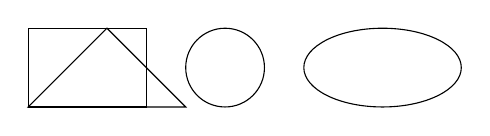
\begin{tikzpicture}
        \draw (0,0) -- (1,1) -- (2,0) -- cycle;
        \draw (0,0) rectangle (1.5,1);
        \draw (2.5, 0.5) circle [radius=0.5];
        \draw (4.5,0.5) ellipse [x radius=1, y radius=0.5];
    \end{tikzpicture}
    \begin{tikzpicture}
        \draw (0,0) |- (1,1);
        \draw (1,0) -| (2,1);
        \draw (4,0) arc (0:135:1);
        \draw (6,0) arc (0:135:1 and 0.5);
    \end{tikzpicture}
    
\begin{tikzpicture}
        \draw (0,0) sin (1,1);
        \draw (0,1) sin (1,0);
        \draw (2,1) cos (3,0);
        \draw (2,0) cos (3,1);
    \end{tikzpicture}
    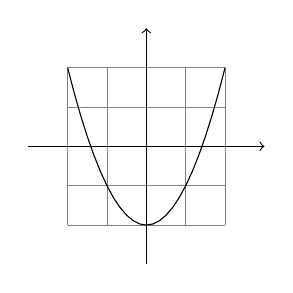
\begin{tikzpicture}
        \draw[help lines,step=0.5] (-1,-1) grid (1,1);
        \draw[->](-1.5,0)--(1.5,0);
        \draw[->](0,-1.5)--(0,1.5);
        \draw[domain=-1:1] plot(\x,{\x*\x*2-1});
    \end{tikzpicture}
    \tikz \filldraw[fill=yellow,draw=red] (2,0.5) circle [radius=0.5];
    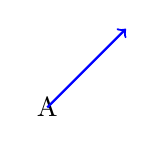
\begin{tikzpicture}
        [myarrow/.style={blue,thick,->}]
        \node (A) at (0,0) {A};
        \draw[myarrow] (0,0)--(1,1);
    \end{tikzpicture}
    use tikzset to set
    

\end{document}
